\chapter{Introduction to Common Intermediate Language}
\section{CIL Fundamentals}
The way CIL code get written are arranged by stack. So assume we have the following code in C\#:
\lstinputlisting[style=customcs]{codes/Chap7/Chap7Snippet1.cs}
That code would be compiled as follow:
\lstinputlisting[style=customcs]{codes/Chap7/Chap7Snippet2.cs}

There are few things happening here:
The shorthand CIL opcode, "ldarg.0", loads the first parameter, int a, to the stack. "ldarg.0" is a short hand opcode that you do not have to specify an argument for which parameter to load after opcode, so it save space and serves as a shortcut for runtime to infers what operation to build for that opcode.

Then "ldarg.1" do a similar operation to the above, but load the second parameter onto the stack. The "add" operation requires no arguments, but it pop off 2 items off the stack, so in "add" opcode point of view, when it pop the stack, it would see "ldarg.1" first and then "ldarg.0" second, this is something to keep in mind if you were to plan on writing a new runtime. The "add" opcode will arrange the items that were popped off the stack and do an addition operation from there (it uses the left-hand value type for addition) and then push the result of the addition to the stack.

Now that we have one remaining item in our stack, the "ret" opcode will pop the item off the stack and return that value for function return value.
\newpage
In an effort to help you actually be able to visualize and understand how this works:

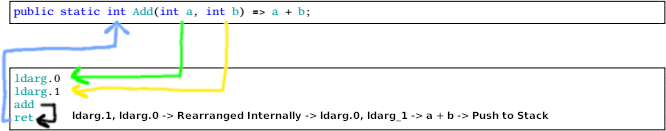
\includegraphics[width=\textwidth]{ChapSevenVisual}